\documentclass[aspectratio=169]{beamer}
%% Choose aspect ratio and other standard options:
% [aspectratio=169] % 16:9 (default)
% [aspectratio=43]  % 4:3 

\usetheme[institute]{tugraz2018}
%% Choose main theme variant:
% [standard]        % standard (default)
% [institute]       % with institute's graphical acronym on the left
% [minimal]         % with reduced visuals

%% Choose your font style:
%                   % Helvetica (default for Corporate Design)
% [webfont]         % Source Sans Pro (as used on tugraz.at)
% [nofont]          % no font loaded - Computer Modern Sans

%% For more options, see README.pdf

\usepackage[utf8]{inputenc}
\usepackage[english]{babel}
%% Choose your main language:
% [ngerman]   % German
% [english]   % English


%% Add your own packages, macros, etc.
% ...


%% Enter presentation metadata
\title[Short Title]{ Hierarchical architectures for spiking \\ Winner-Take-All networks}
\author{Christoph Rieger, \\ Supervisor: Univ.-Prof. Dipl.-Ing. Dr.techn. Robert Legenstein
}
\date{10.01.2025}
\institute{IML}
\instituteurl{www.iml.tugraz.at}

%% Logos
\institutelogo{beamerthemetugraz/institute/igi}  % graphical acronym for [institute] theme (left margin)
% \additionallogo{figures/logo}  % additional institute/department logo (footline; optional)
%\logobar{Supervisor: Univ.-Prof. Dipl.-Ing. Dr.techn. Robert Legenstein
%}  % sponsors (titlepage; optional)


\begin{document}

\begin{frame}[plain]
  \maketitle
\end{frame}


\begin{frame}{Outline}
  \tableofcontents
\end{frame}


\section{Introduction}

\begin{frame}{Biological background}
  \begin{columns}[onlytextwidth]
	\begin{column}{0.7\textwidth}
	\vspace{-1.0cm}
      \begin{itemize}
        \item Spiking neural networks
        \begin{itemize}
          \item Resemble biological neural networks closely
          \item Generate and propagate neural spikes
        \end{itemize}
        \item Winner-Take-All networks
        \item Probabilistic brain
        \item Synaptic plasticity
      \end{itemize}
	\end{column}
	\begin{column}{0.3\textwidth}
      \begin{figure}
        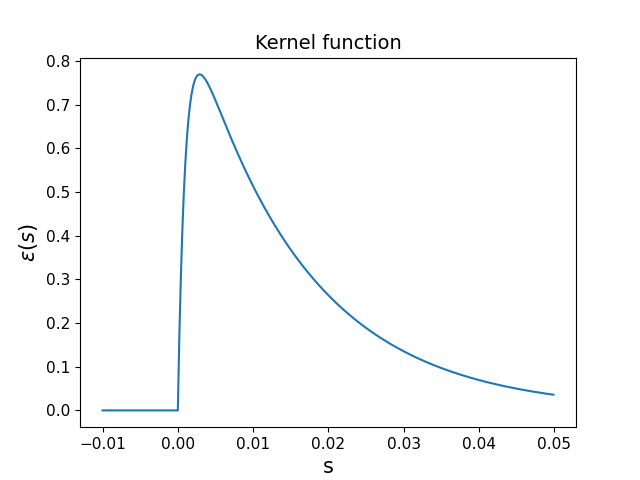
\includegraphics[width=1\linewidth]{../Latex/figures/kernelFunction.png}
      \end{figure} 
  	\end{column}
  \end{columns}
\end{frame}

\begin{frame}{Biological background}
  \begin{columns}[onlytextwidth]
	\begin{column}{0.7\textwidth}
	\vspace{-1.0cm}
      \begin{itemize}
        \item Networks are organized in hierarchical structure
        \item Feedback used for attention / biased competition
        \item Lee and Mumford found that feedback could let neurons see illusory contour
   \end{itemize}
	\end{column}
	\begin{column}{0.3\textwidth}
      \begin{figure}
        
\includegraphics[width=0.6\linewidth]{../Latex/figures/kanizsaSquare.PNG}
      \\   \footnotesize Kanizsa square, Source: Lee and Mumford
      \end{figure} 
  	\end{column}
  \end{columns}
  \scriptsize Source: Lee T.S., Mumford D. (2003), “Hierarchical Bayesian inference in the
 visual cortex.”, In: J Opt Soc Am A Opt Image Sci Vis
\end{frame}

\begin{frame}{Theoretical background}
\vspace{-1.0cm}
      \begin{itemize}
        \item Bayesian inference gives the probability of an hypothesis given related evidence
        \item $P(Y = k|X, Z) = \frac{P(X|Y=k)P(Y = k|Z)}{\Sigma_{k'}P(X|Y=k')P(Y=k'|Z)}$
        \item Model of Nessler et al. expanded by prior neuron layer
          \begin{itemize}
            \item Proved mathematically that expansion is valid
          \end{itemize}
        \item Nessler et al. claimed that synaptic input weights converge towards the log of likelihood, $w^{I}_{ki} = log(P(x_i = 1 | Y = k))$
        \end{itemize}
   \scriptsize Source: Nessler et al. (2013), “Bayesian Computation Emerges in
 Generic Cortical Microcircuits through Spike-Timing-Dependent Plasticity.”, In: PLOS Computational Biology 9.4
\end{frame}

\begin{frame}{The network}
  \begin{columns}[onlytextwidth]
	\begin{column}{0.5\textwidth}
	  \begin{itemize}
	    \item $u_k(t) = \sum_{i=1}^N w^{I}_{ki} \cdot x_i(t) + \sum_{j=1}^J w^{P}_{kj} \cdot z_j(t)$
	    \item $p(y_k \text{ fires at time t}) \propto e^{u_k(t) - I(t)}$
	    \item $w^{I}_{ki} = log(P(x_i = 1 | Y = k))$
	    \item $w^{P}_{kj} = log(P(Y = k | Z = j))$
	  \end{itemize}
    \end{column}
    \begin{column}{0.5\textwidth}
        \begin{figure}
        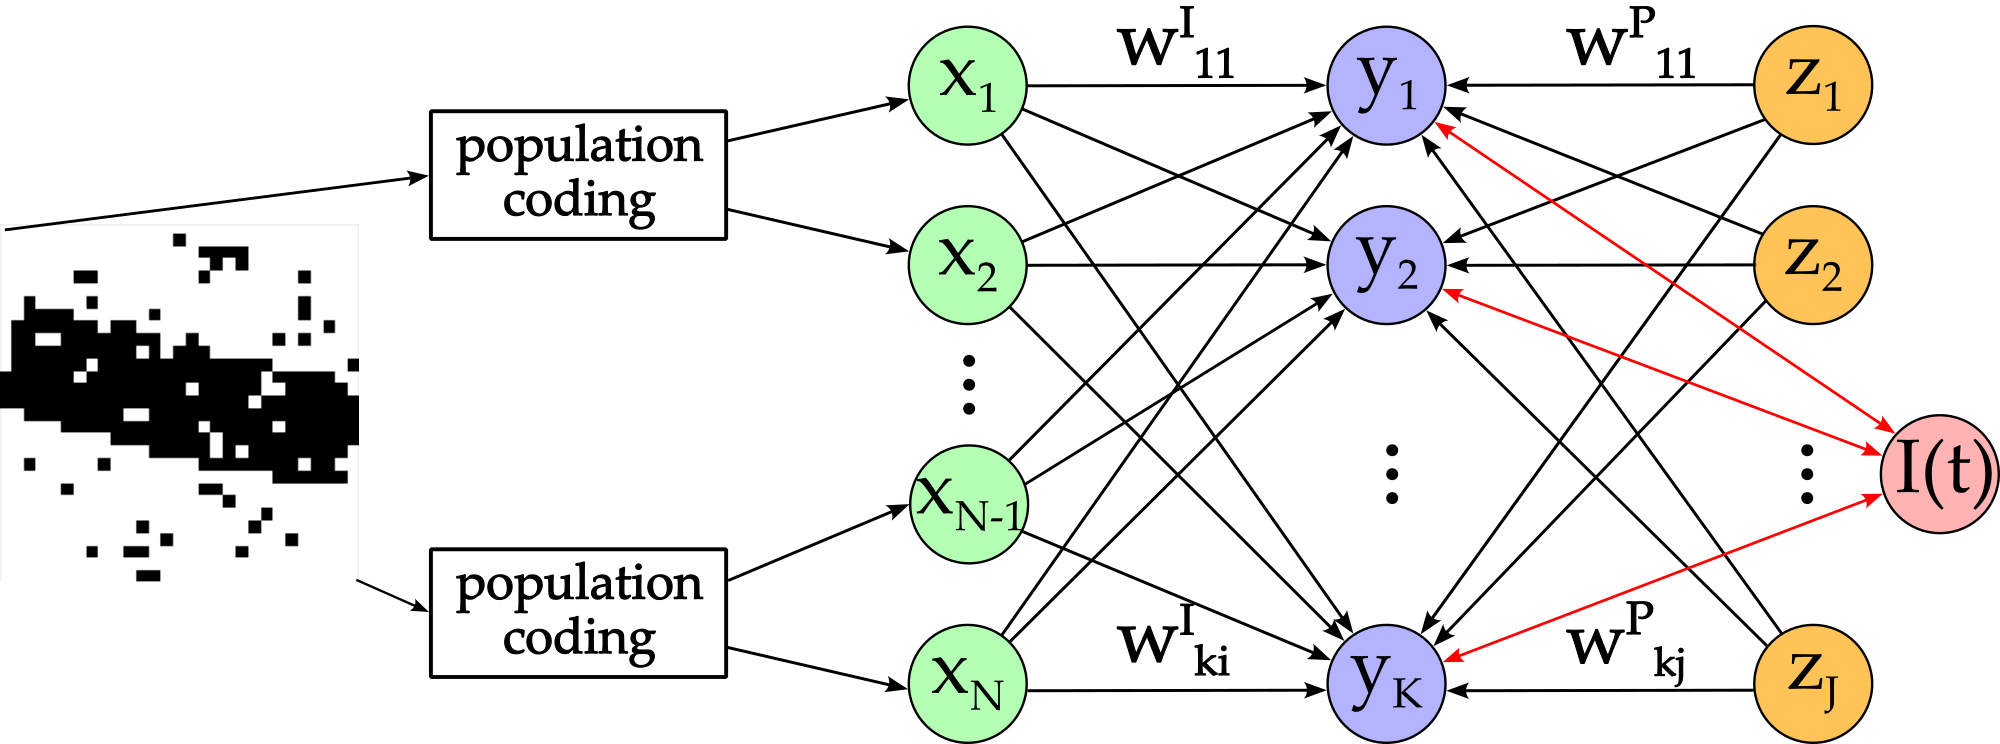
\includegraphics[width=1\linewidth]{../Latex/figures/networkPlan.png}
      \end{figure} 
	\end{column}
  \end{columns}
\end{frame}

\begin{frame}{Goals}


  \begin{itemize}
  %  \item $e^{learned\: input\: weights}$
   % \item $e^{learned\: prior\: weights}$
    %\item $e^{calculated\: input\: weights}$
    %\item $e^{calculated\: prior\: weights}$

    \item Increase the understanding of the network model
    \item Simulate feedback found in the visual cortex
    \item Show connection between Bayesian inference and network model
  \end{itemize}
\end{frame}


\section{Experiments}

\begin{frame}{Methodology}
\begin{itemize}
	\item Simulation was performed in Python
	\item Simulation step size was 1 ms
	\item Pixels of input images and the prior had a noise level of 10\%
	\item Kullback-Leibler divergence was chosen to evaluate performance of model
	\begin{itemize}
	  \item Compared firing rates of output neurons to analytical Bayesian posterior
	\end{itemize}
\end{itemize}
\end{frame}

\begin{frame}{Ambiguous visual stimuli 1}
  \begin{itemize}
    \item Network learned to group horizontal and vertical bars into 10 groups
    \item After training ambiguous images with 1 horizontal and 1 vertical bar were shown
    \item Network was able to focus on individual bars, due to prior neurons
  \end{itemize}
\end{frame}

\begin{frame}{Ambiguous visual stimuli 2}
\vspace{-1.0cm}
        \begin{figure}
        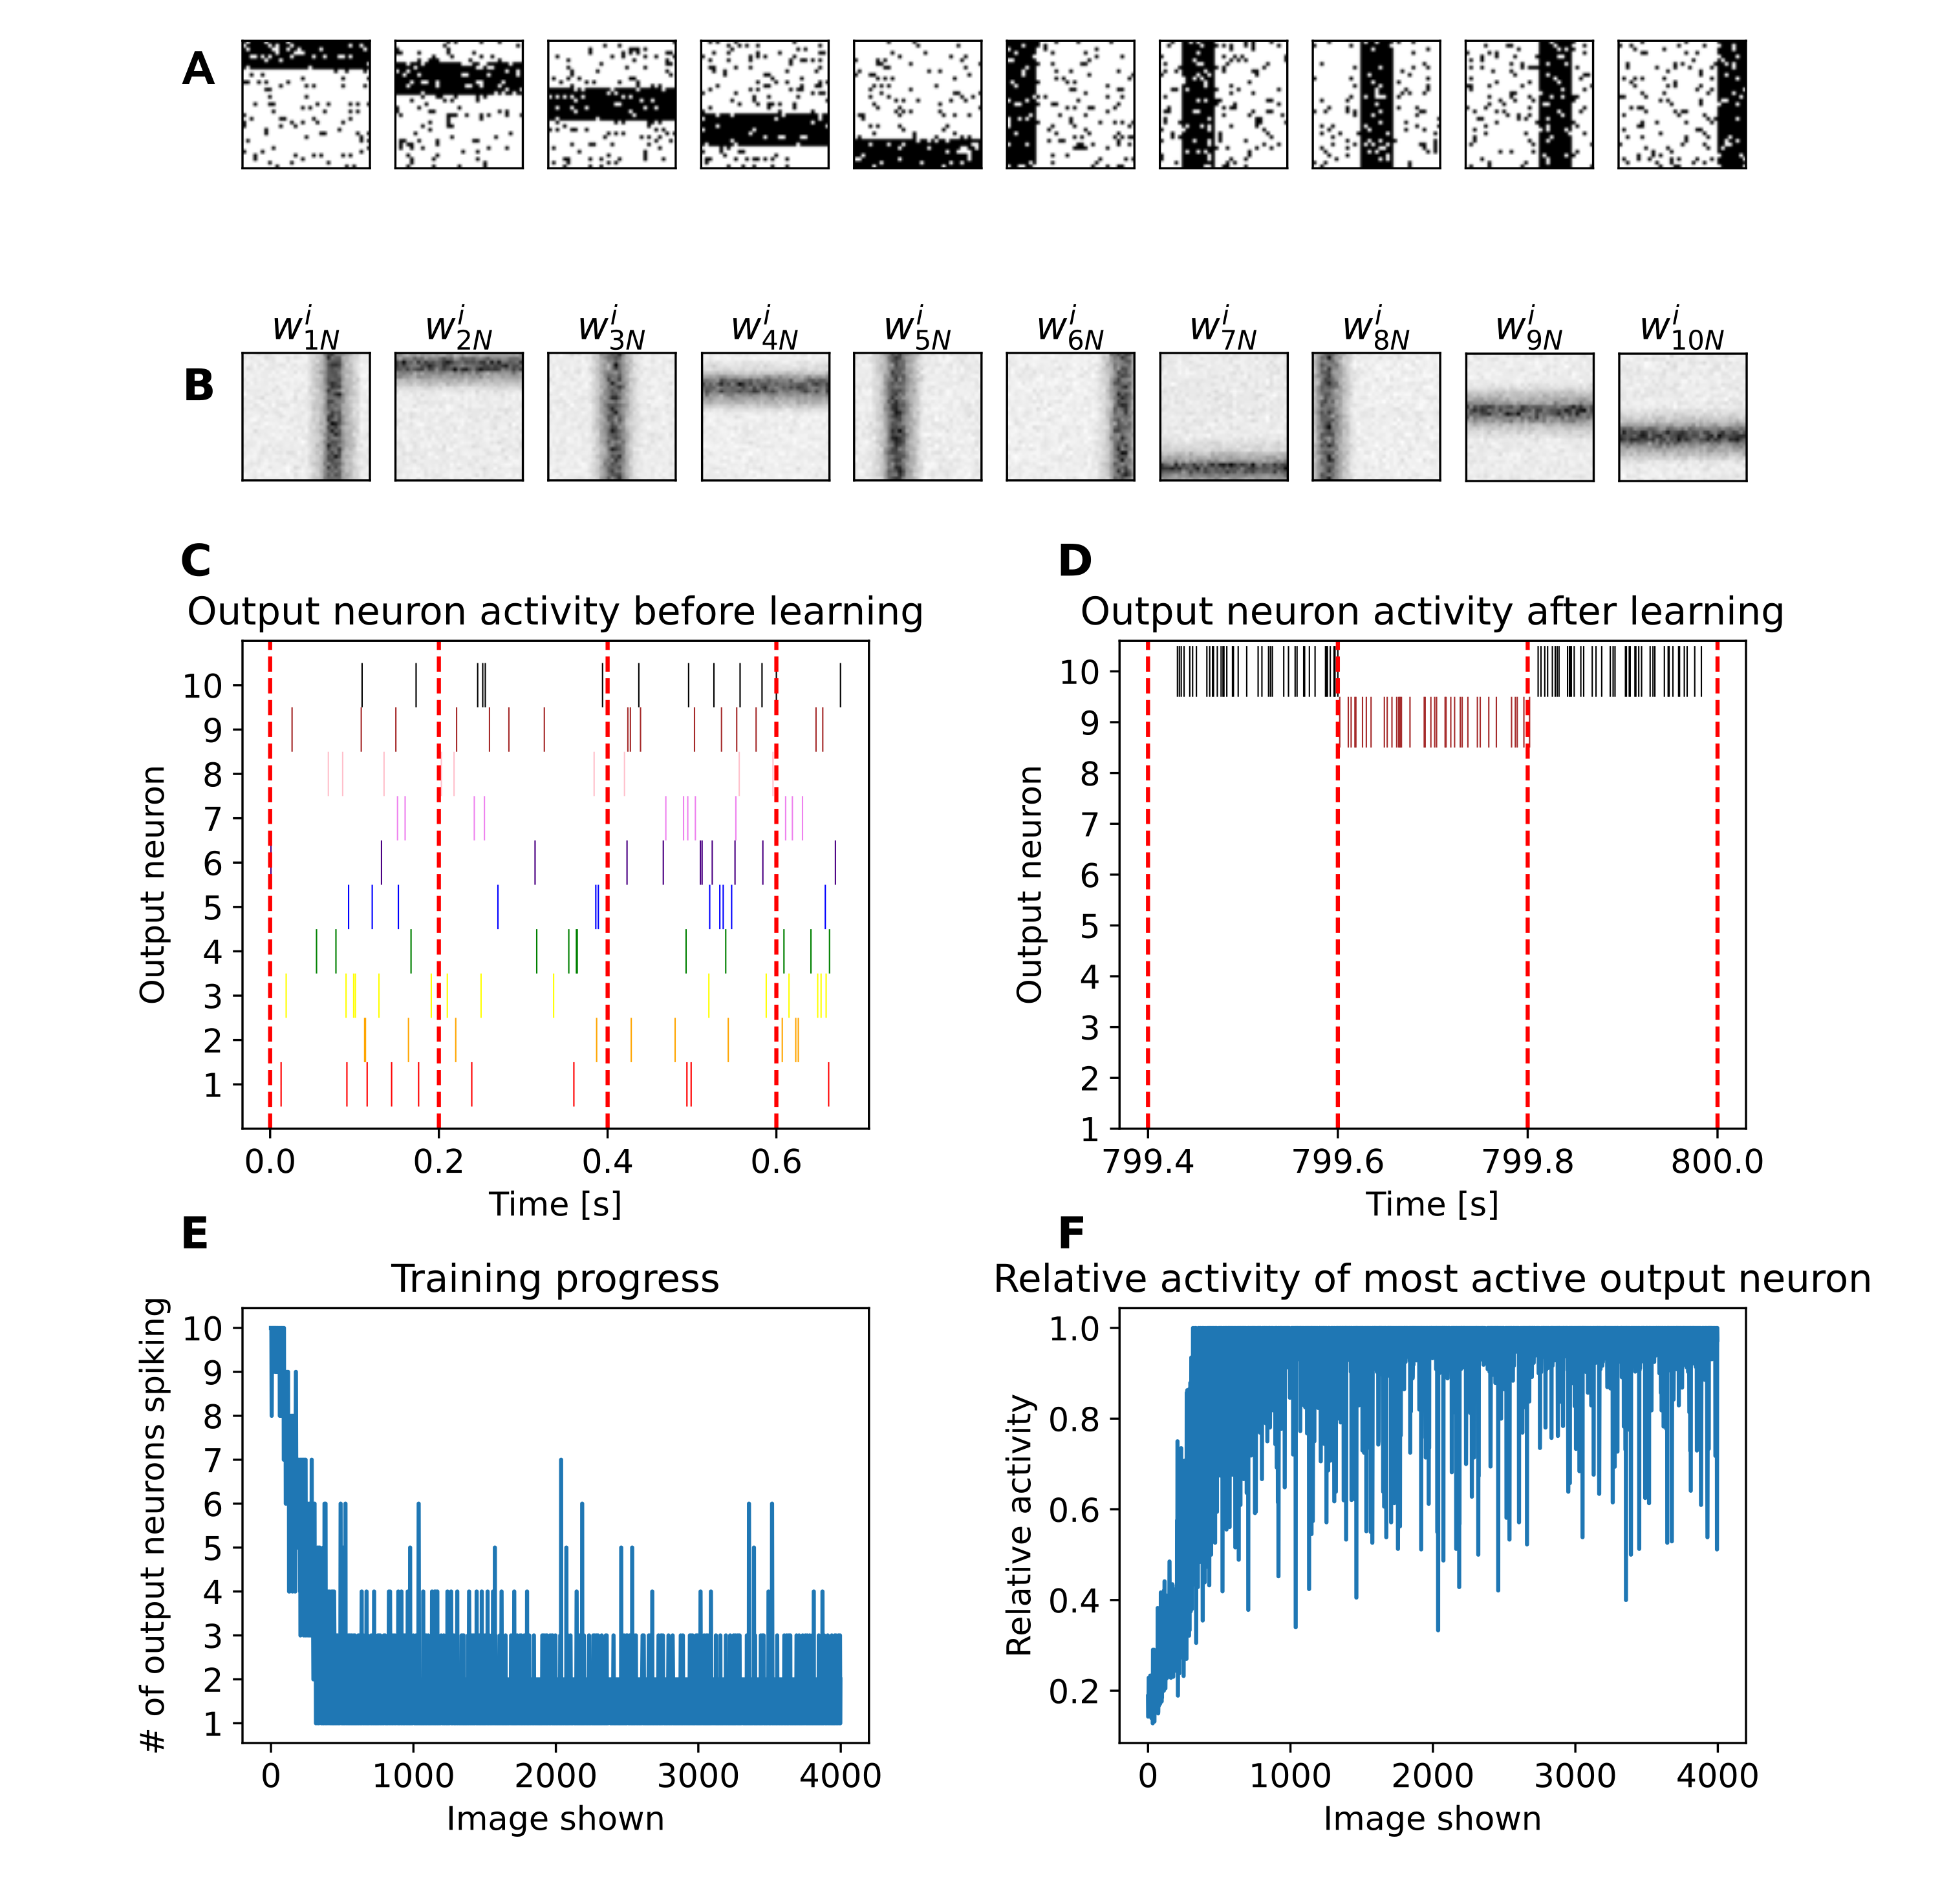
\includegraphics[width=0.40\linewidth]{../Latex/figures/horvertAdaptiveInh/trainingPlotCropped.png}
      \\   \footnotesize Training plot
      \end{figure} 
\end{frame}

%\begin{frame}{Ambiguous visual stimuli 3}
%   \begin{columns}[onlytextwidth]
%	\begin{column}{0.5\textwidth}
%	 \vspace{-1.5cm}
%	        \begin{figure}
 %       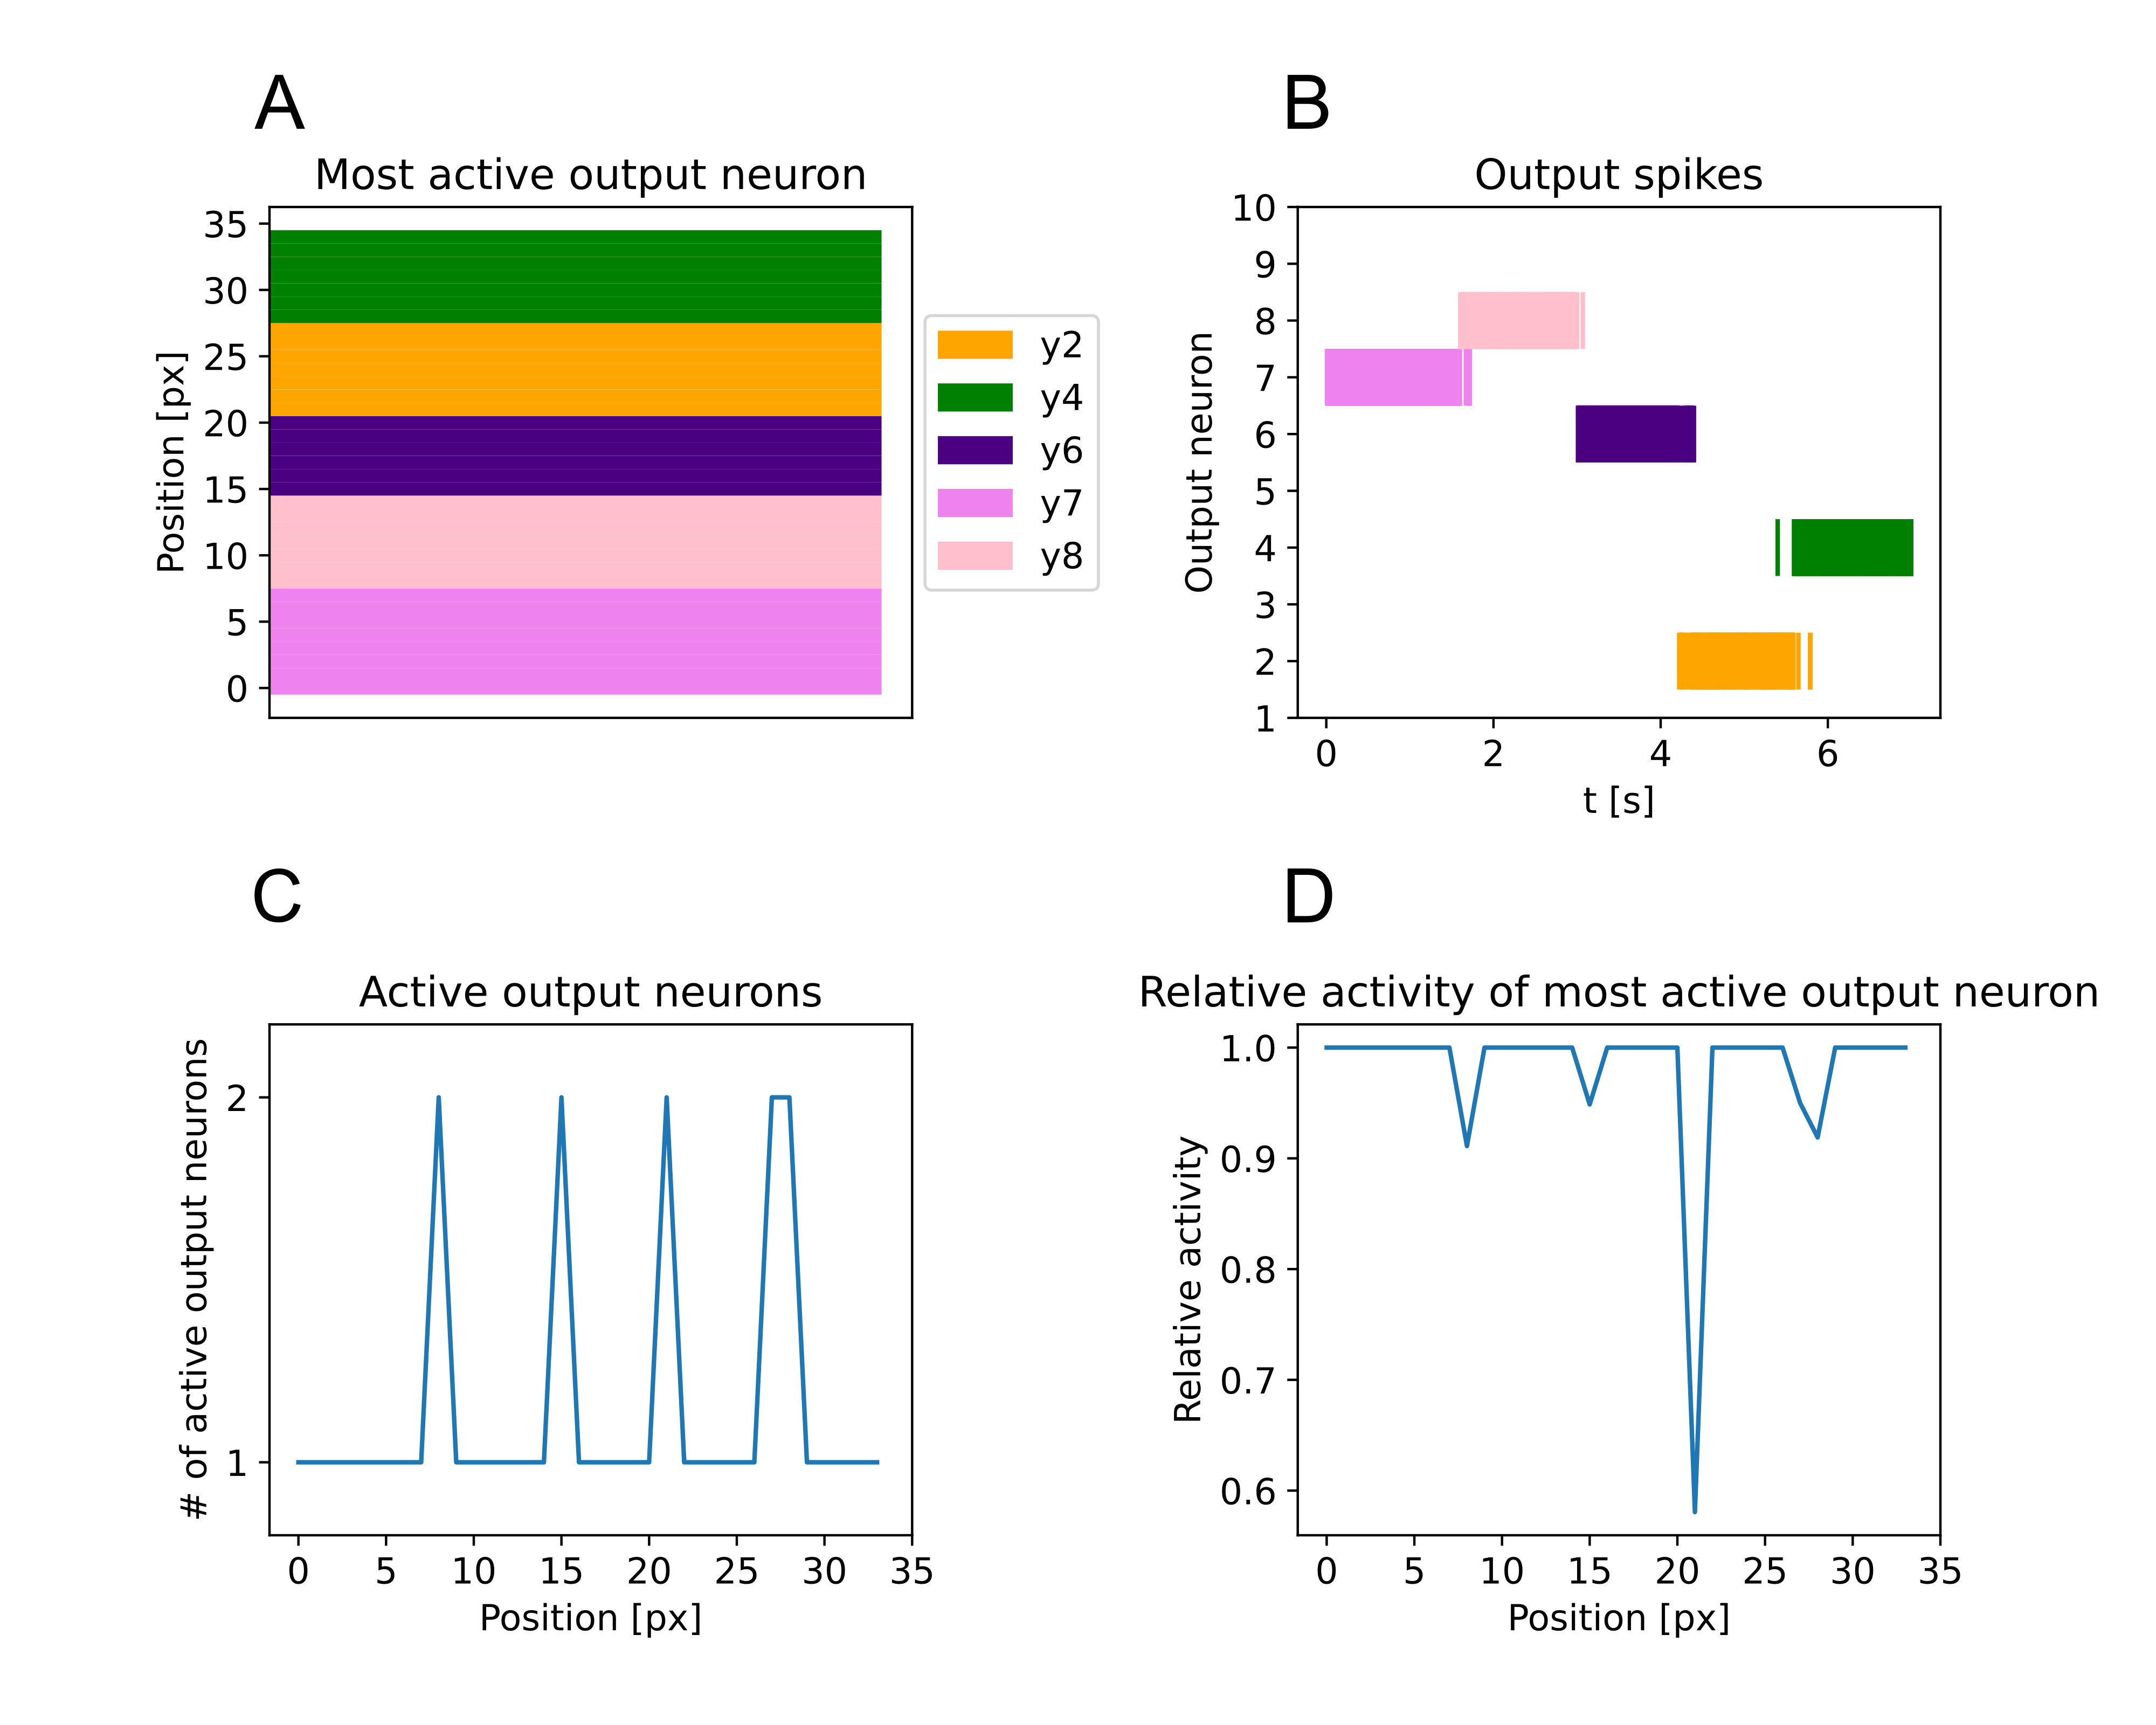
\includegraphics[width=0.8\linewidth]{../Latex/figures/horvertAdaptiveInh/horizontal_validation.png}
%      \\   \scriptsize Horizontal validation
%      \end{figure} 
%	\end{column}
%	\begin{column}{0.5\textwidth}
%	\vspace{-1.5cm}
%		        \begin{figure}
 %       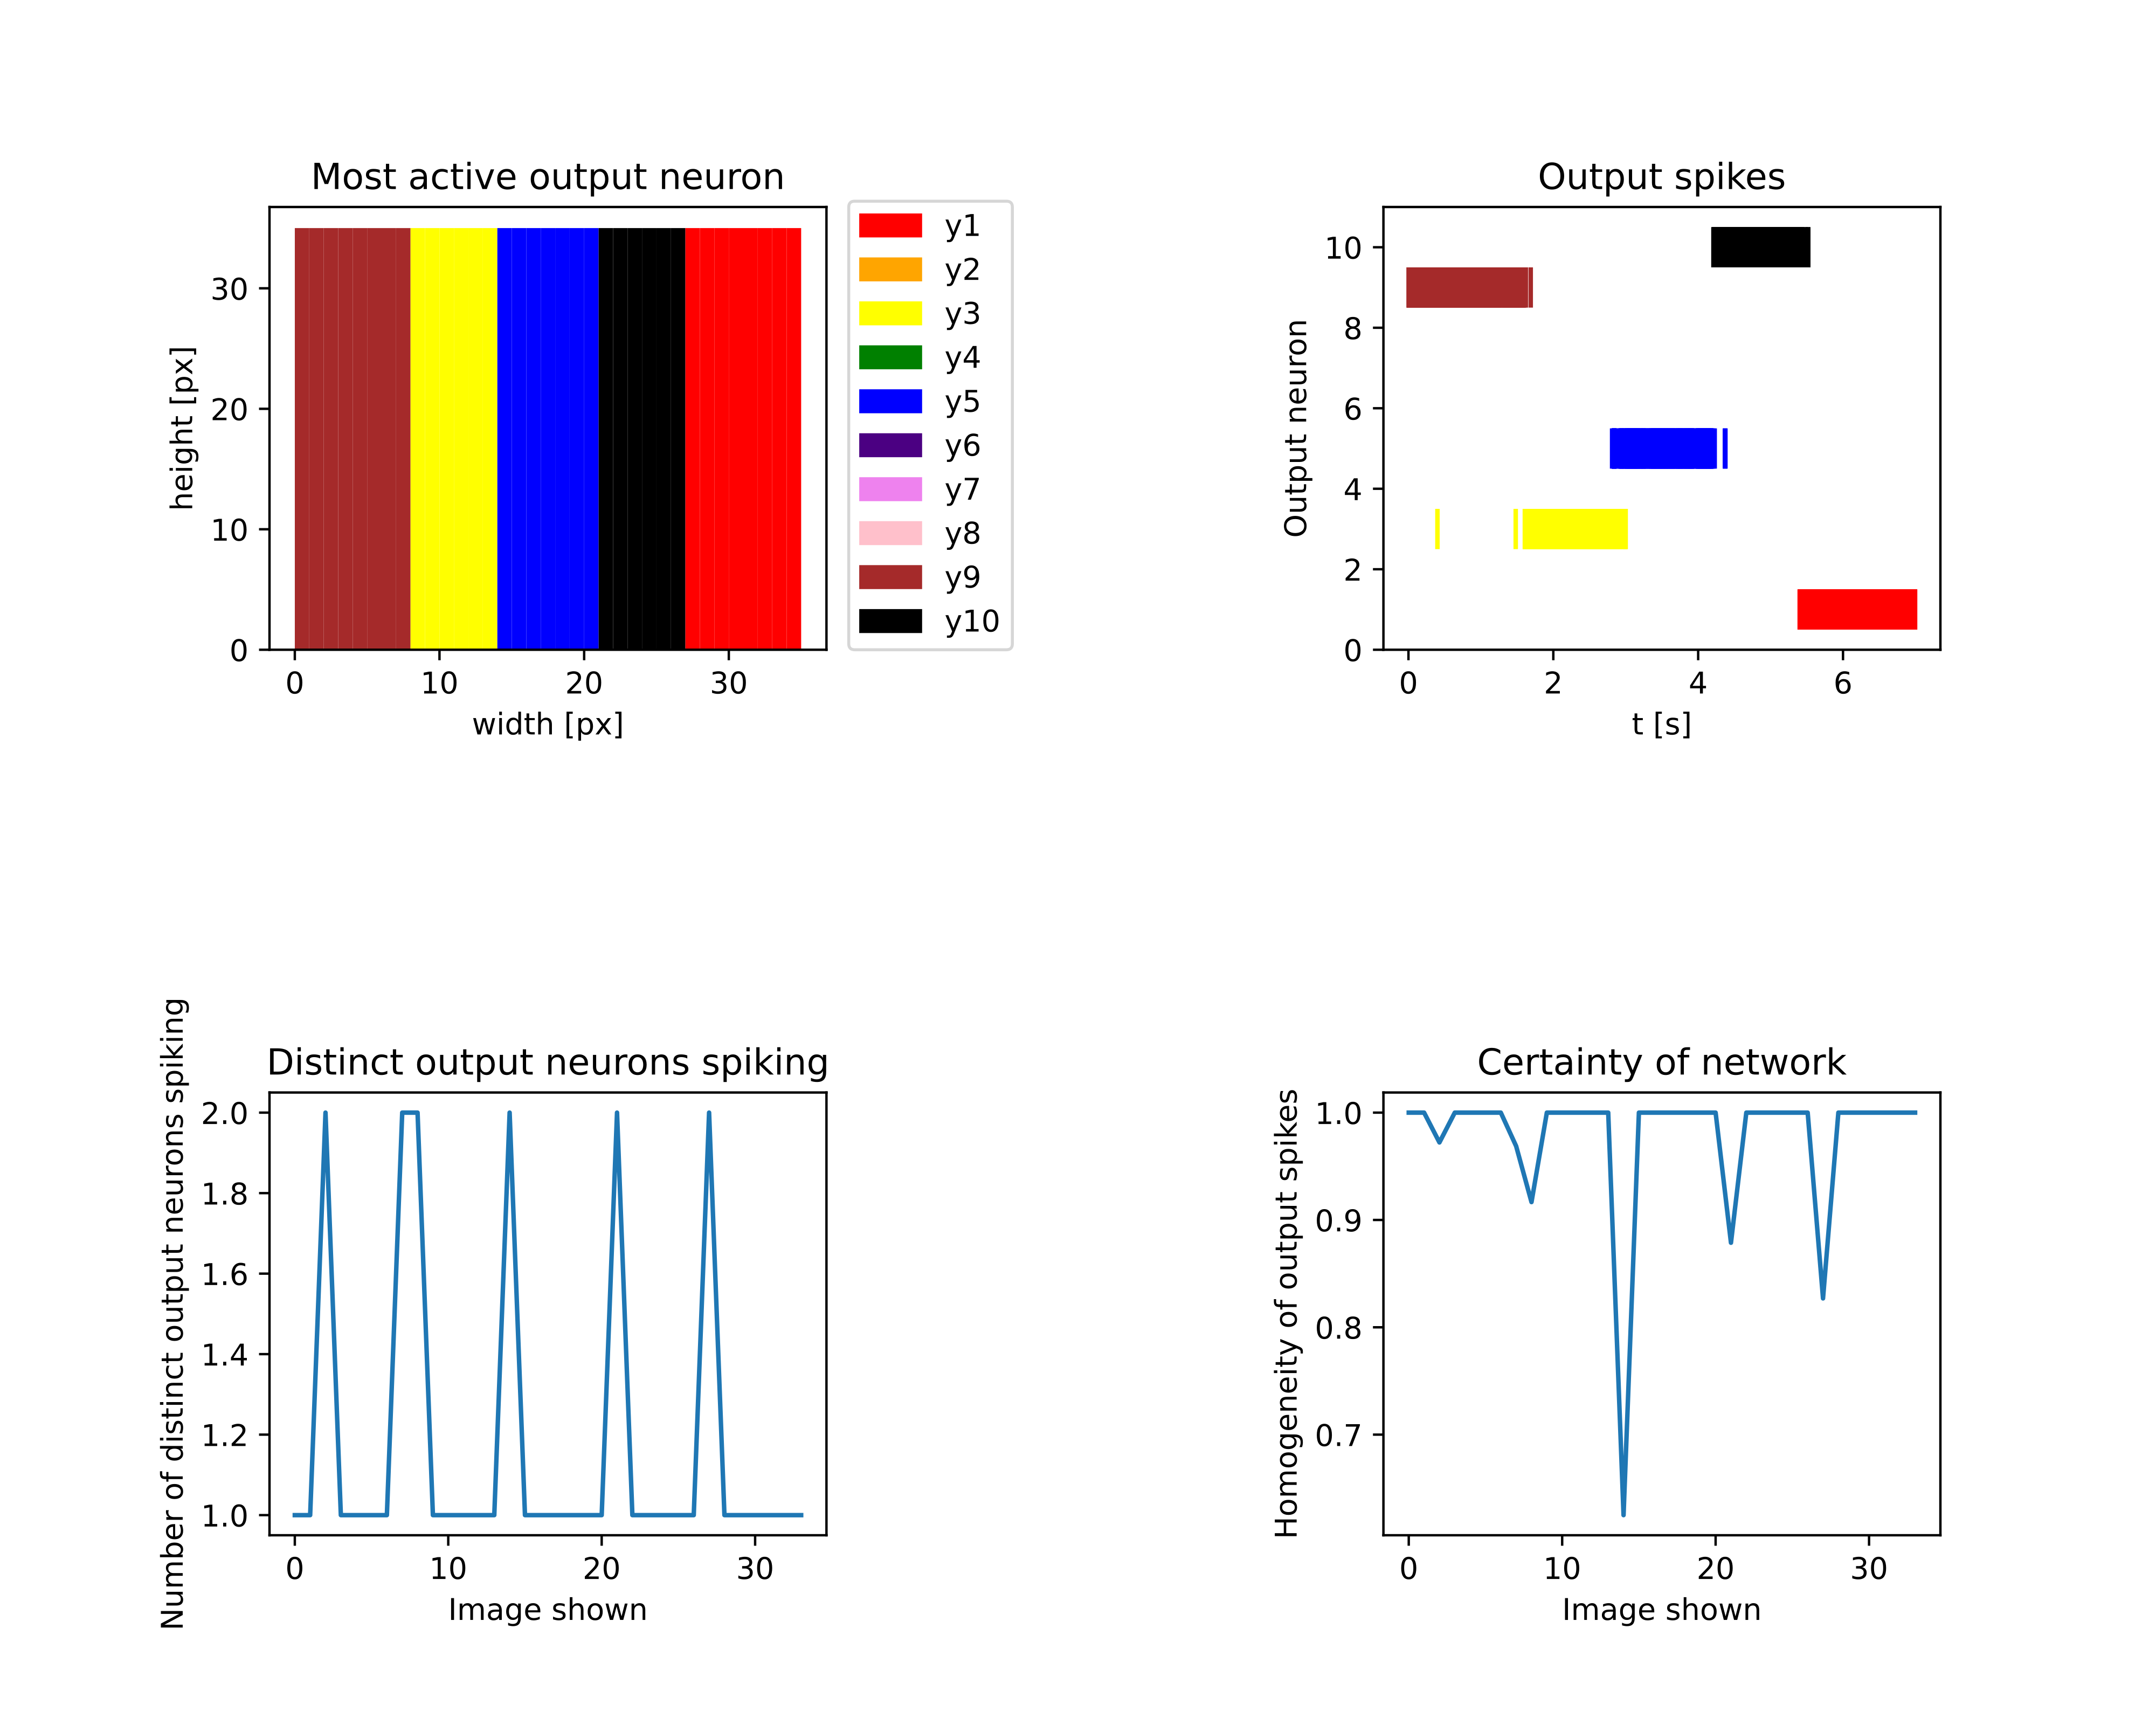
\includegraphics[width=0.8\linewidth]{../Latex/figures/horvertAdaptiveInh/vertical_validation.png}
  %    \\   \scriptsize Vertical validation
  %    \end{figure} 
%	\end{column}
 % \end{columns}
%\end{frame}

\begin{frame}{Ambiguous visual stimuli 3}
		\begin{figure}
        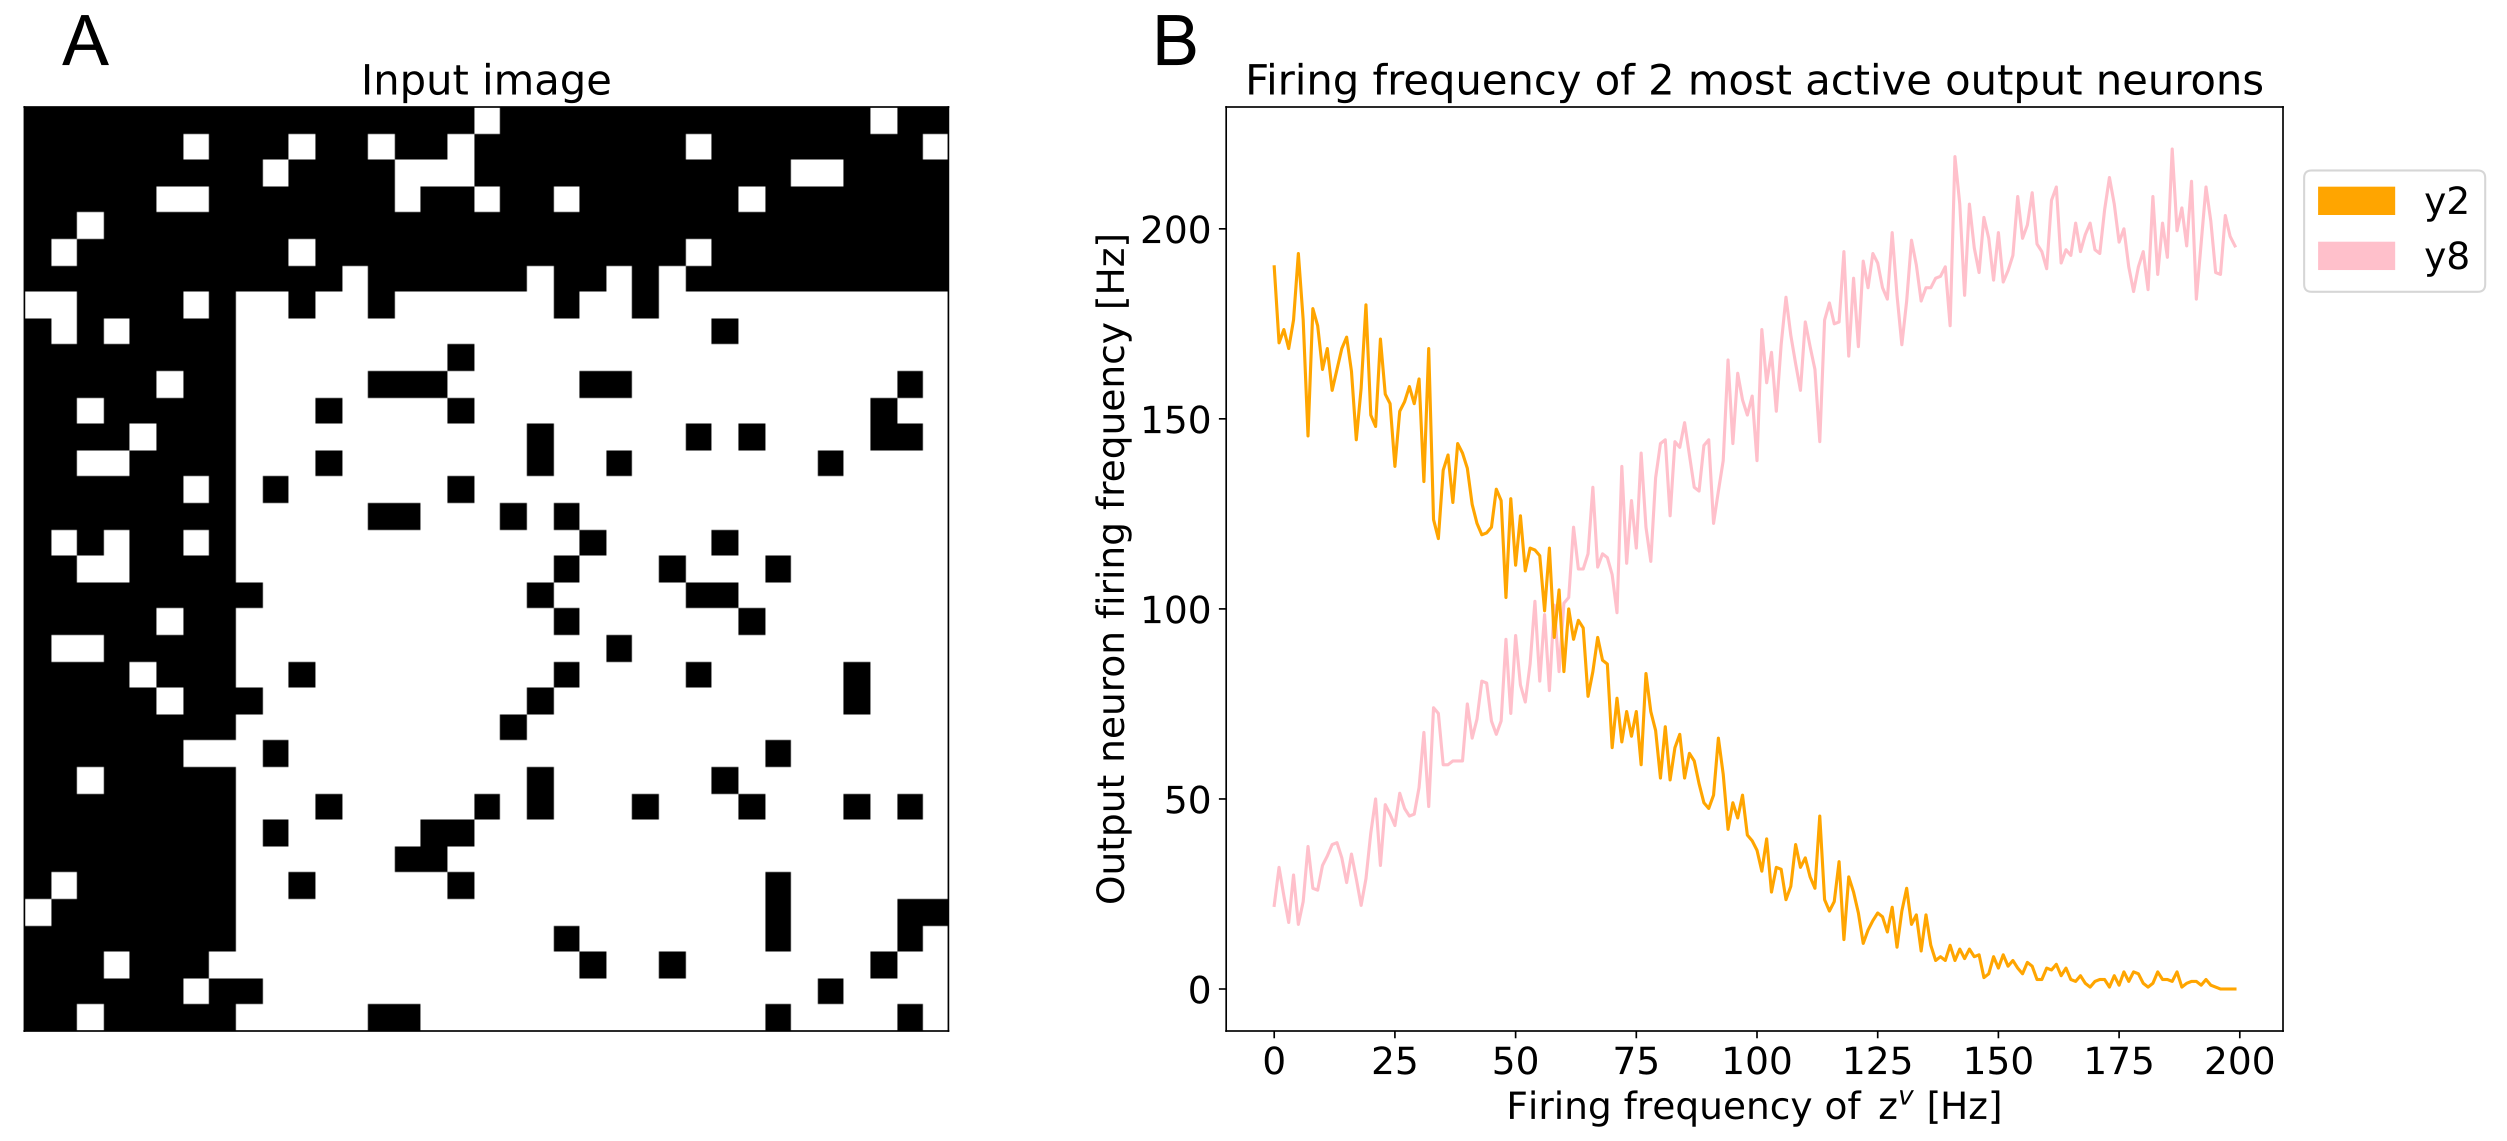
\includegraphics[width=0.7\linewidth]{../Latex/figures/horvertAdaptiveInh/YFrequency_prior.png}
      \\   \scriptsize Variable prior activity
      \end{figure} 
\end{frame}

\begin{frame}{Analysis and
 simulation of the network 1}
	\begin{itemize}
	  \item Usage of smaller 1-D images to make network easier to analyse 
	  \item Mathematical derivation of Bayesian likelihood, prior and posterior
	  \item Derived synaptic weights from Bayesian likelihood and prior
	  \item Simulated network with those weights and fitted hyperparameters
	  \item Compared Bayesian posterior to output of the simulation
	\end{itemize}
\end{frame}

\begin{frame}{Analysis and
 simulation of the network 2}
 \vspace{-1.0cm}
		\begin{figure}
        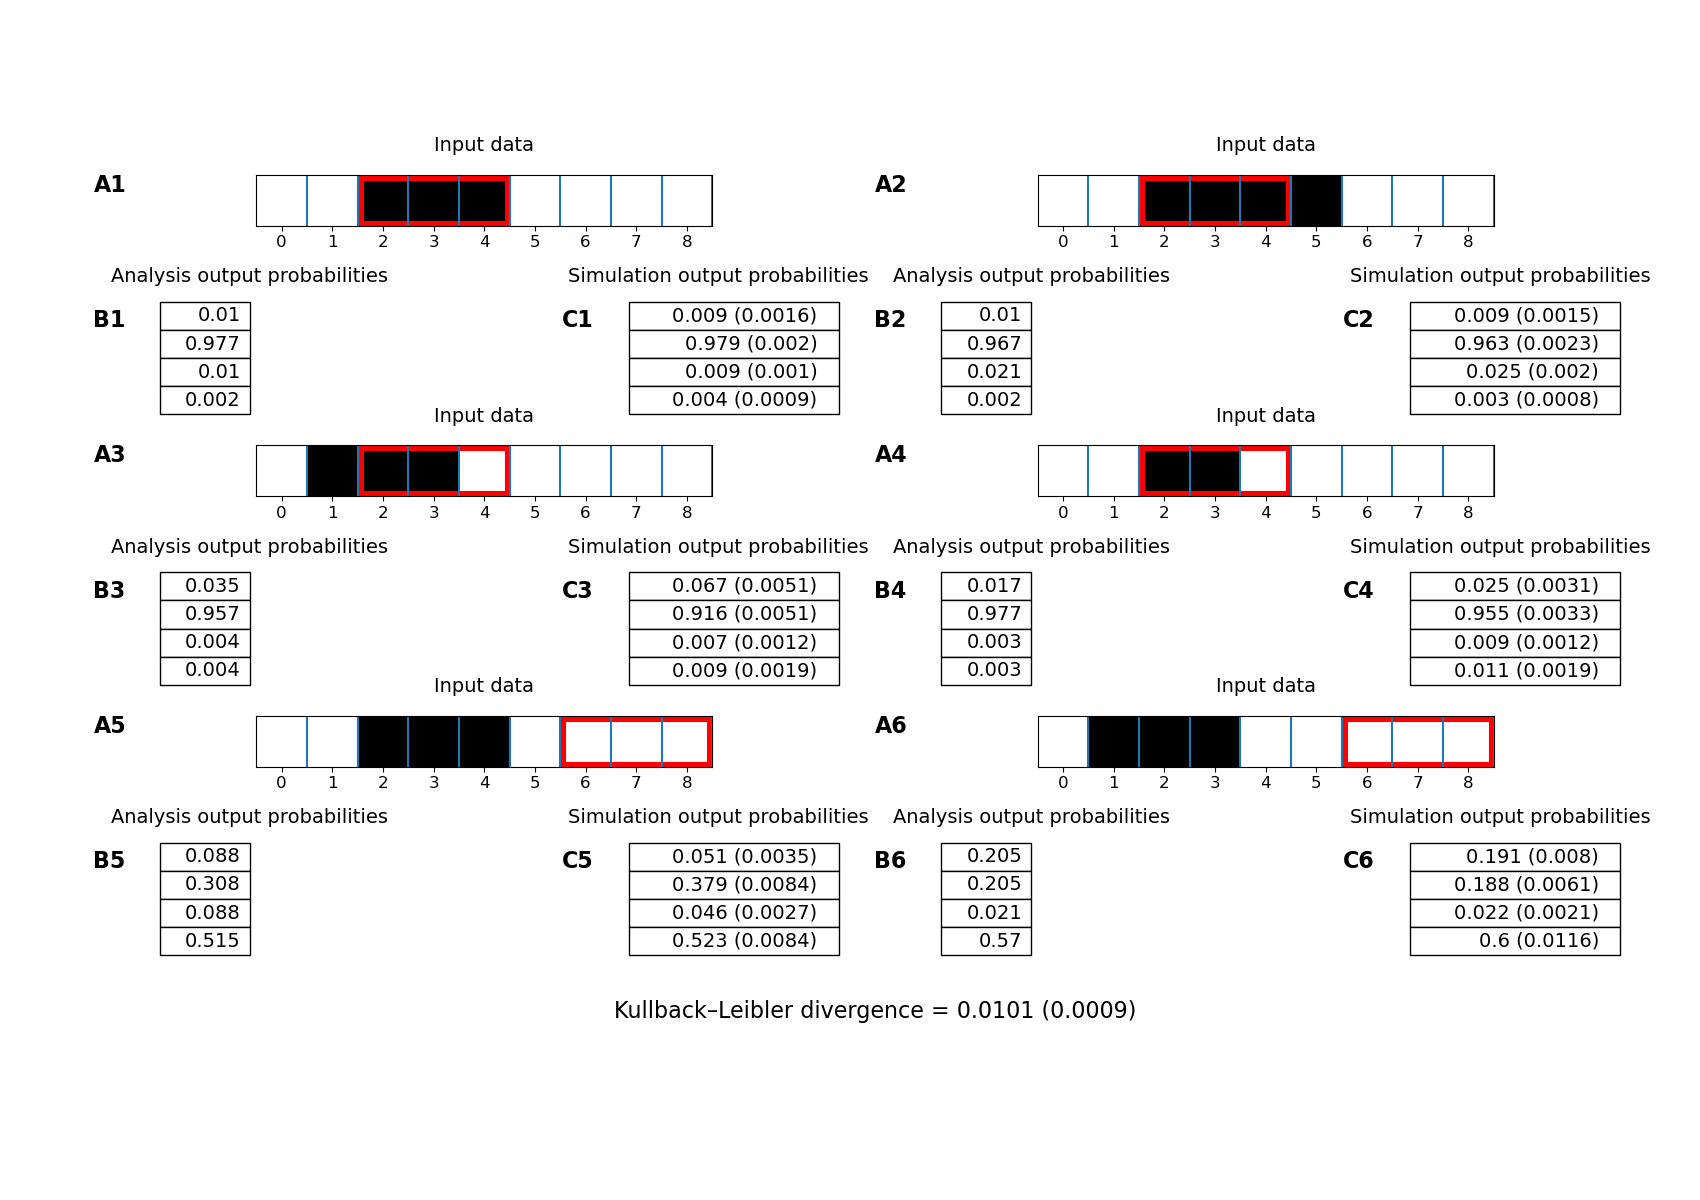
\includegraphics[width=0.35\linewidth]{../Latex/figures/1D/1D_98_440_4.png}
      \end{figure} 
\end{frame}

\begin{frame}{Transferability of hyperparameters 1}
  \begin{itemize}
      \item Network was simulated with same hyperparameters of smaller network, to check if they are applicable to any network size
    \item Input size and prior neuron firing rate  was doubled
  \end{itemize}
\end{frame}

\begin{frame}{Transferability of hyperparameters 2}
 \vspace{-1.0cm}
		\begin{figure}
        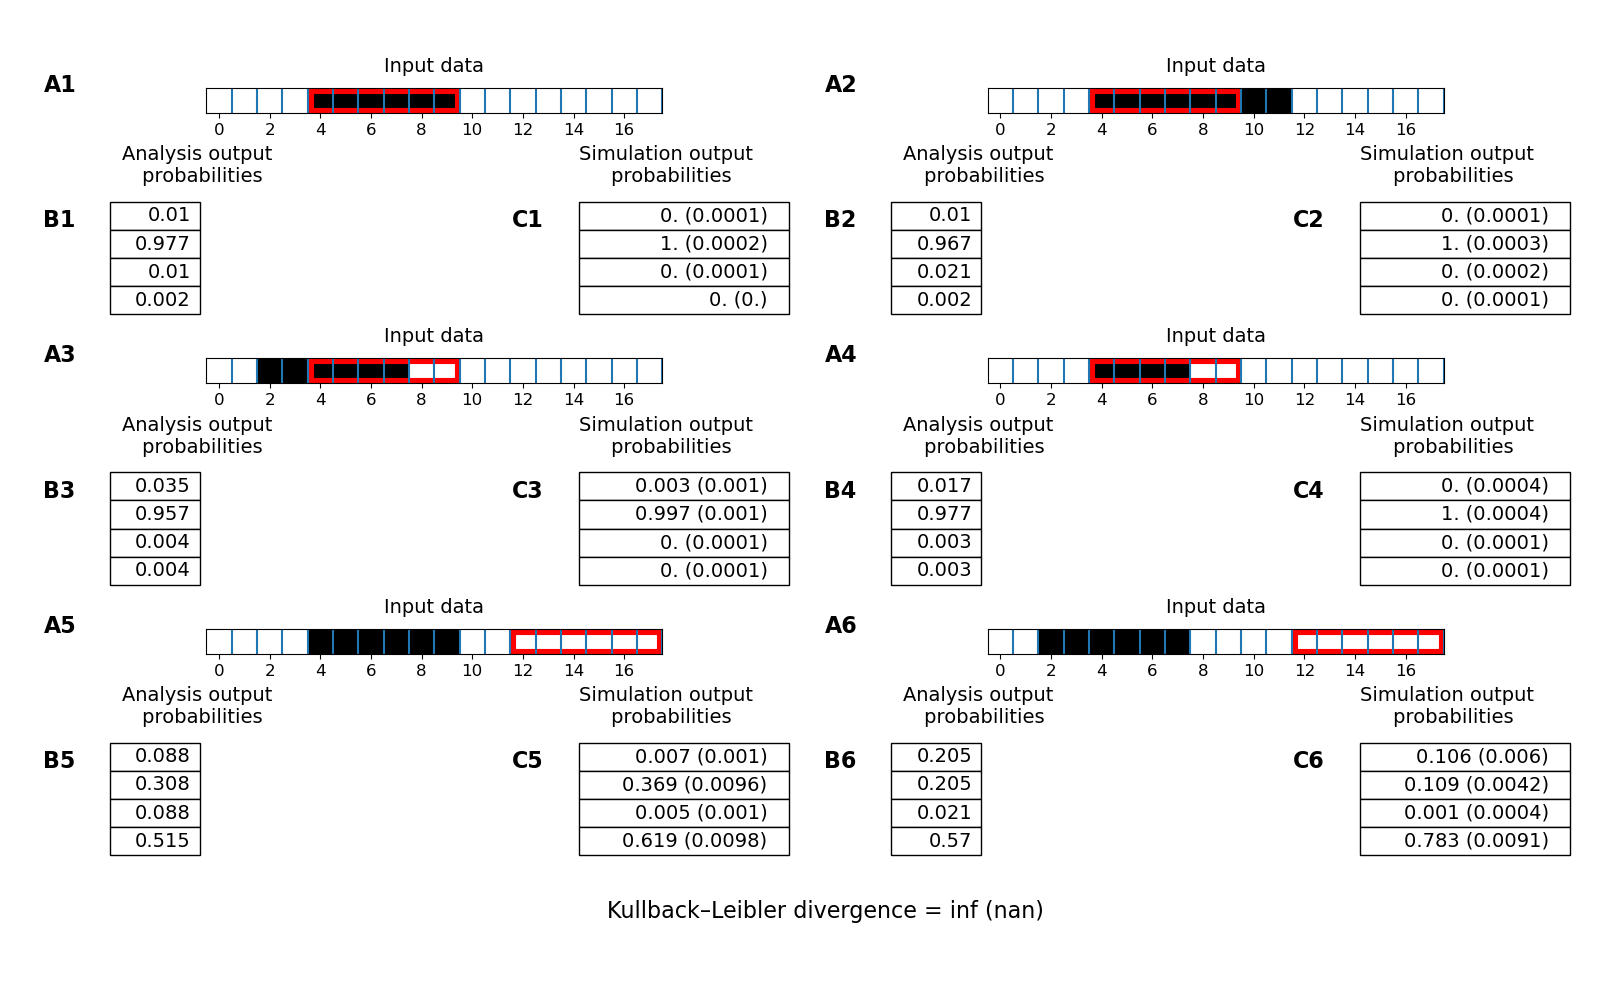
\includegraphics[width=0.4\linewidth]{../Latex/figures/1D/doubleSize/doubleSize_98_880_4.png}
      \end{figure} 
\end{frame}



\begin{frame}{Training with predetermined hyperparameters 1}
  \begin{itemize}
    \item Determined hyperparameters were used to train weights
    \item Trained weights were compared to analytically determined weights
  \end{itemize}
\end{frame}

\begin{frame}{Training with predetermined hyperparameters 2}
 \vspace{-1.0cm}
		\begin{figure}
        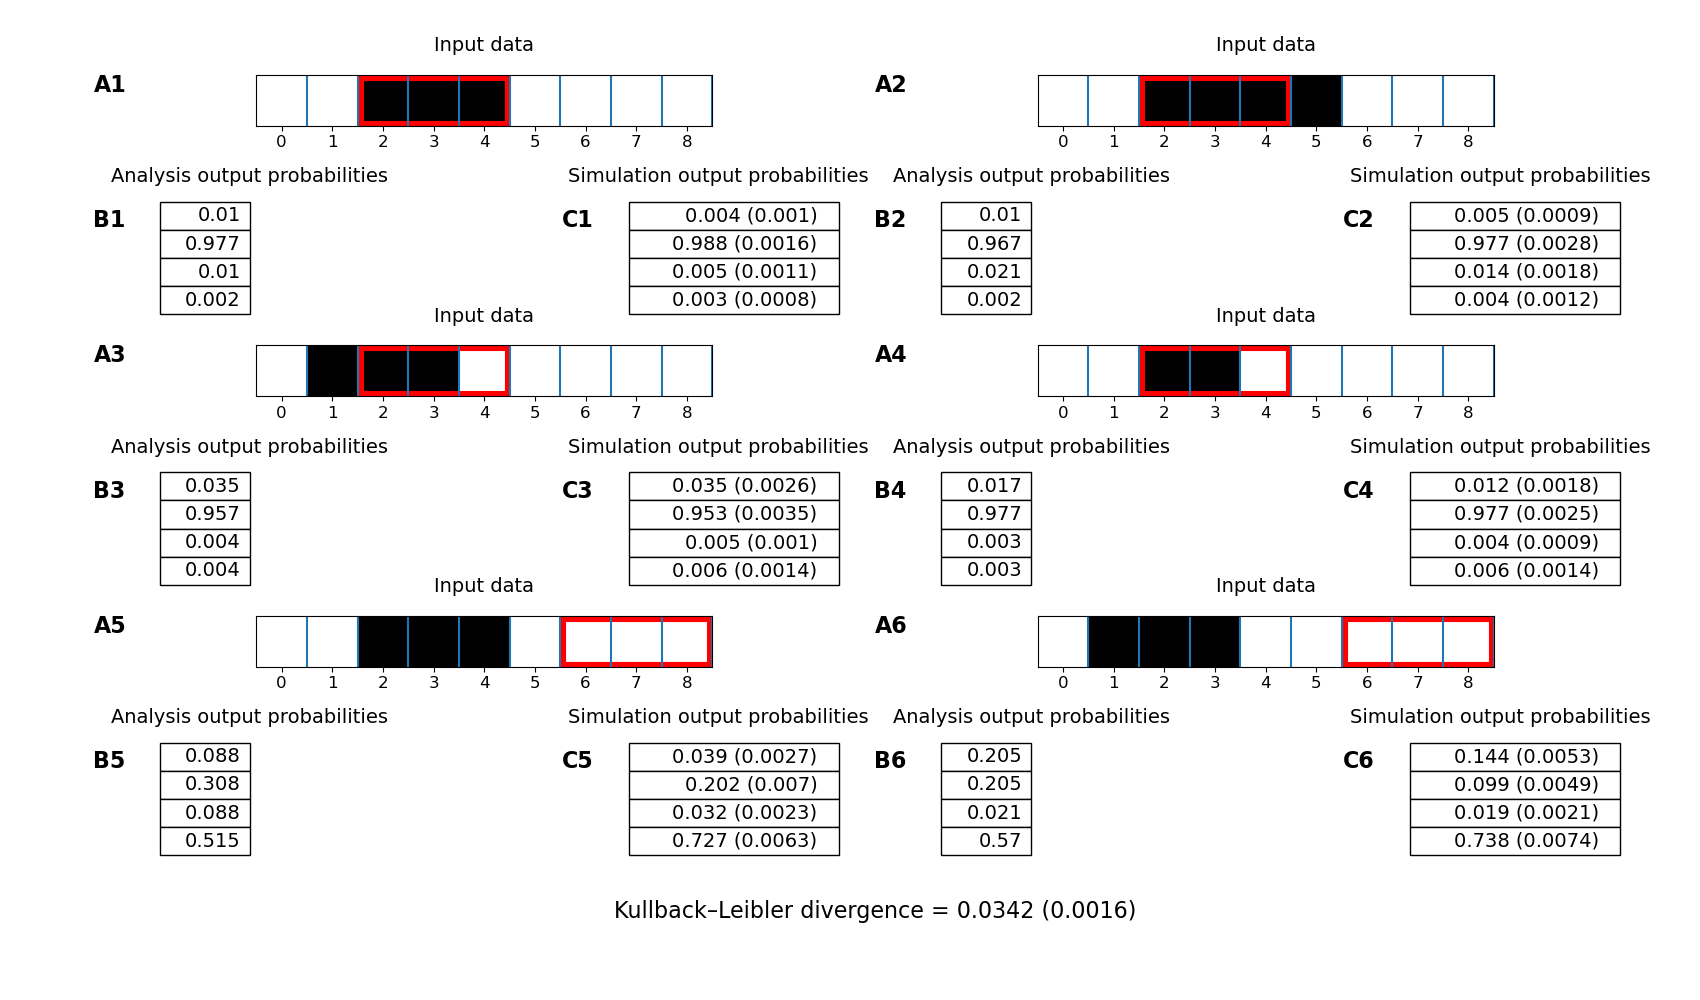
\includegraphics[width=0.35\linewidth]{../Latex/figures/1D/training/trainingEvaluation_98_440_4_c3.png}
      \end{figure} 
\end{frame}

\begin{frame}{Training with predetermined hyperparameters 3}
 \vspace{-1.0cm}
		\begin{figure}
        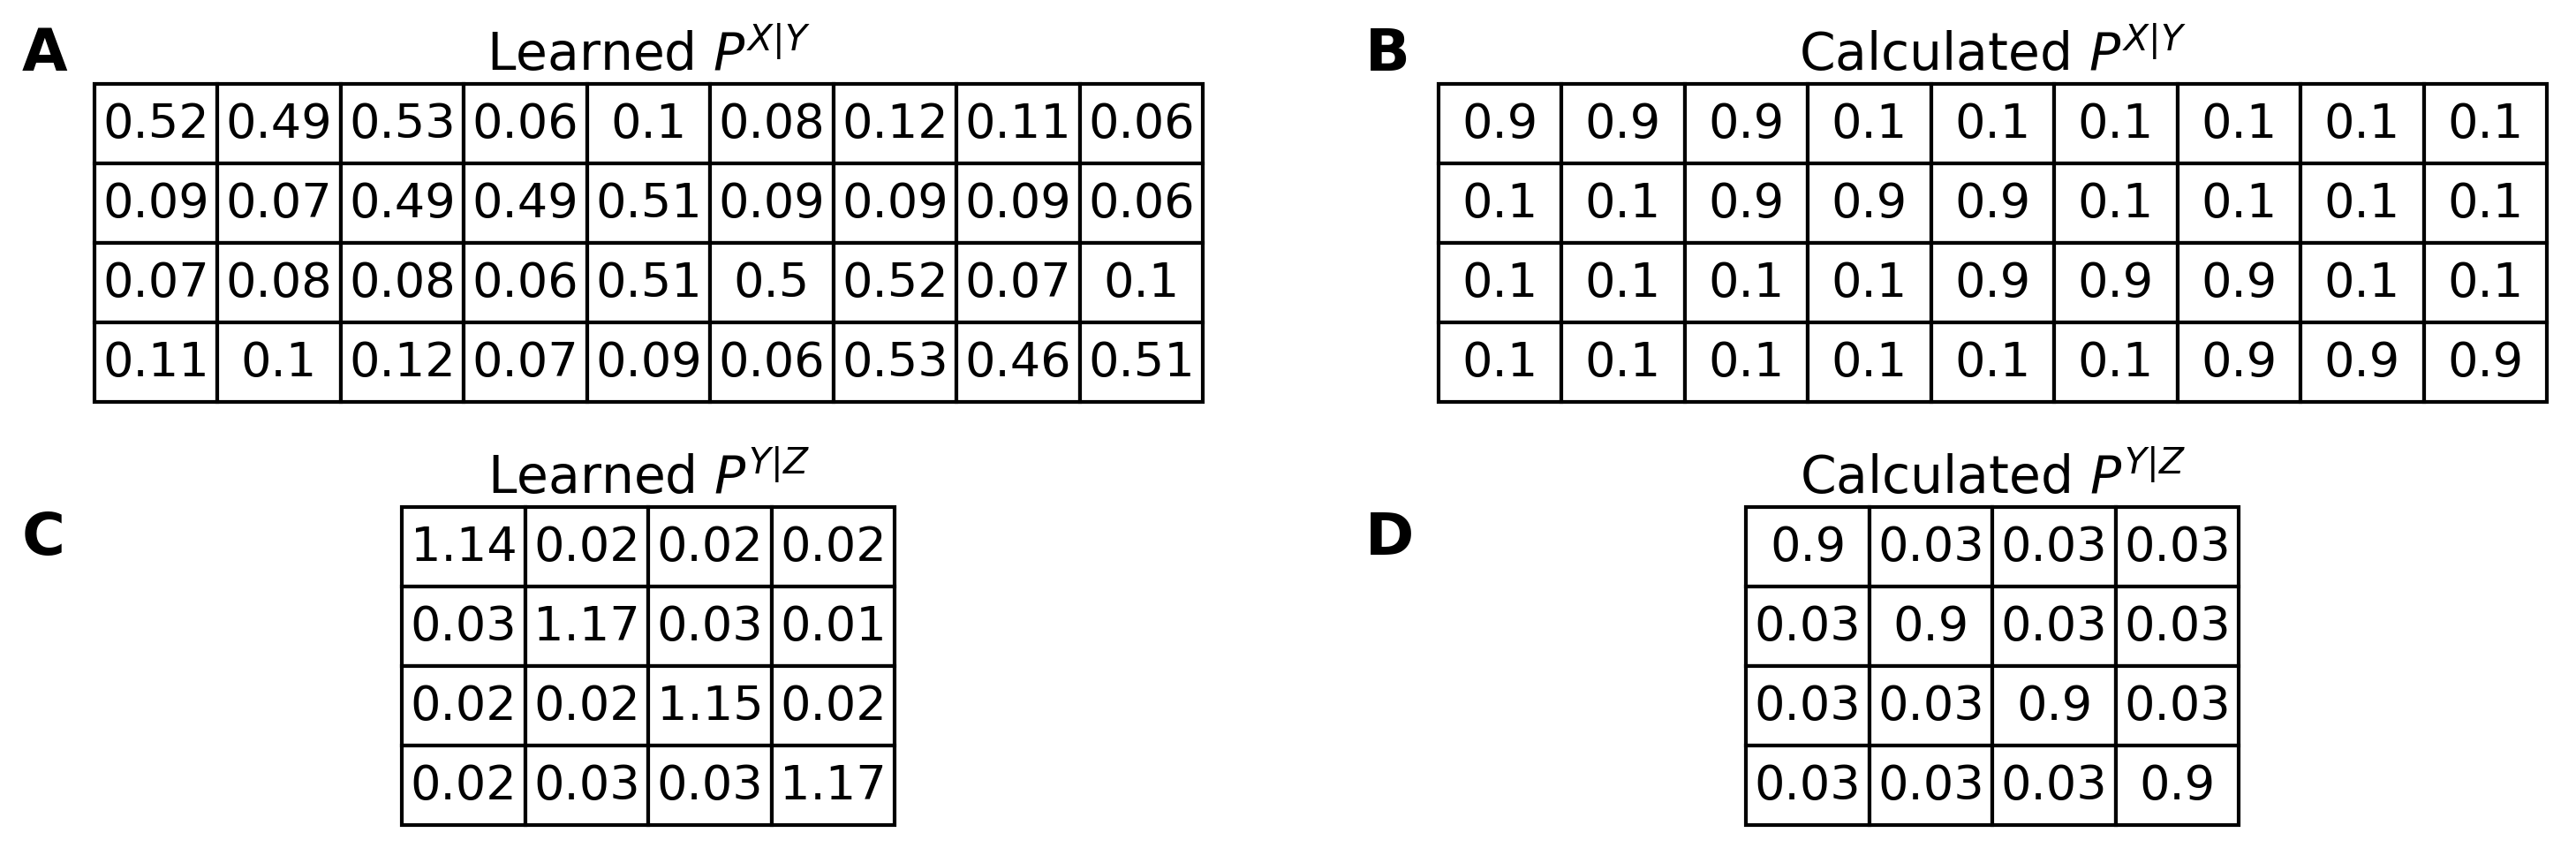
\includegraphics[width=0.7\linewidth]{../Latex/figures/1D/training/weightComparison.png}
      \end{figure} 
\end{frame}

\section{Results}

\begin{frame}{Results}
	\vspace{-0.5cm}
    \begin{itemize}    
    \item Connection between model and Bayesian inference was shown
    \begin{itemize}
      \item Network outputs spikes according to Bayesian posterior
      \item Trained weights converge towards the log of their respective probabilities
    \end{itemize}
    \item Importance of neural feedback was shown for 
    \begin{itemize}
	  \item Attention / Ambiguity resolution
	  \item Illusory contour effect
    \end{itemize}   
  \end{itemize}
\end{frame}

\begin{frame}{Results}
  \begin{itemize}
      \item Optimal hyperparameters are dependent on network size
    \item Training process could not achieve perfectly trained weights 
  \end{itemize}
\end{frame}

\section*{Conclusion}

\begin{frame}{Conclusion}
  \begin{itemize}
	\item Thesis provided insight to hierarchical spiking Winner-Take-All network model
	\item Showed that the network model can simulate effects like attention and changing beliefs through feedback
	\item Provided ideas on how to further analyse and improve the model
  \end{itemize}
\end{frame}


\begin{frame}{Sources}
    \begin{itemize}
    \item  Lee T.S., Mumford D. (July 2003). “Hierarchical Bayesian inference in the
 visual cortex.” In: J Opt Soc Am A Opt Image Sci Vis. DOI: doi:10.1364/josaa.20.001434
    \item Nessler, Bernhard et al. (Apr. 2013). “Bayesian Computation Emerges in
 Generic Cortical Microcircuits through Spike-Timing-Dependent Plasticity.” In: PLOS Computational Biology 9.4, pp. 1–30. doi: 10.1371/journal.
 pcbi.1003037. url: https://doi.org/10.1371/journal.pcbi.1003037
  \end{itemize}

\end{frame}

\end{document}
